\documentclass{article} % For LaTeX2e
\usepackage{nips13submit_e,times}
\usepackage{hyperref}
\usepackage{epsfig}
%\usepackage{mahnig}
\usepackage{url}
\usepackage{enumerate}
\usepackage{booktabs}
\usepackage{graphicx}

%\documentstyle[nips13submit_09,times,art10]{article} % For LaTeX 2.09




\title{Parkinson Detection}
\author{Jon Perez Etxebarria}
% The \author macro works with any number of authors. There are two commands
% used to separate the names and addresses of multiple authors: \And and \AND.
%
% Using \And between authors leaves it to \LaTeX{} to determine where to break
% the lines. Using \AND forces a linebreak at that point. So, if \LaTeX{}
% puts 3 of 4 authors names on the first line, and the last on the second
% line, try using \AND instead of \And before the third author name.
\newcommand{\fix}{\marginpar{FIX}}
\newcommand{\new}{\marginpar{NEW}}
\nipsfinalcopy % Uncomment for camera-ready version
\begin{document}
\maketitle
\begin{abstract}
In this report I will explain the thought process and the implementation of the various solutions to the Parkinson detection from spiral drawings problem. One the bigest problems I will try to tackle during this project is how to set up a process in order to surmount the problem of having such an inbalanced dataset and how to manipulate said data.
\end{abstract}

\bigskip
\bigskip
\bigskip

\section{Some key packages}
 
In order to manage and mold the data pandas is essential since all the data points are stored in CSV format. In the same vein glob is very helpful in order to access the directories where the data is stored. Numpy will also provide many utilities.

For the machine learning part tensorflow v.1.15 was used although it is deprecated since that is the version the institution is using. In my particular case since the installed version is the 2.3.1 i suggest you import the library in the following fashion:

import tensorflow.compat.v1 as tf
\smallskip

tf.disable\_v2\_behavior()
\smallskip

Libraries:

\begin{itemize}
  \item Numpy
  \item Tensorflow
  \item Pandas 
  \item Sklearn
  \item Ipython
  \item Glob
\end{itemize}
 
\bigskip

\section{Description of the problem}
 
In this problem we are presented with a very imbalanced dataset consisting of 15 csv files with data from healthy people and 62 csv files with data from people with parkinson, and we are task with: I) Find suitable feature representations for this problem that are very usable for other ML classifiers, II) Implement a NN that is able to surmount the disparagement in the number of instances for each class. As an additional task I will try to use a Restricted Boltzmann Machine in order to find the features.
\bigskip
\bigskip
\bigskip
\bigskip
\bigskip
\bigskip
\bigskip
\bigskip
\bigskip
\bigskip
\section{Approach for feature Selection}
 
 In this section I will explain my thought process in order to solve the unbalanced dataset problem.
 
\subsection{Description of the data}
  The data is separated in different csv files, one for each person. As I mentioned before the dataset is pretty unbalanced with only 15 from 77 files corresponding to healthy people.

Let's dive into how these csvs are written. Each file has 7 different attributes but they don't include the name for any of them. This names can be found in a separate ‘README’ file and are as follow:

\begin{itemize}
  \item X value
  \item Y value
  \item Z value 
  \item Pressure
  \item GripAngle
  \item Timestamp
  \item Test ID
\end{itemize}

\begin{figure}[h!]
  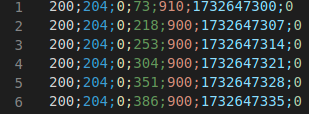
\includegraphics[scale = 1]{csv.png}
  \centering
  \caption{Example from one of the csv files}\hspace*{\fill}
  \label{fig:a}
\end{figure}



Let's get into what each one means since this will be key in order to select the appropriate features from the data. As I mentioned this info was obtained from different types of drawings, this type is what the seventh value refers to.

\begin{itemize}
  \item  0 is de static spiral tes
  \item 1 is the dynamic spiral test
  \item 2 circular motion test
\end{itemize}

The X,Y,Z values refer to the position the pen was relative to the tablet.

The pressure is a measure of how much force the person was applying on the tablet while drawing.

Grip angle is pretty self explanatory, is a reference to the angle the pen was relative to the surface of the tablet.

The timestamp is the time at the moment of registering the data, each value is separated by seven time units.

Now that this is clear let's conclude on what I have. It is pretty obvious that I have a time series for each patient. Realizing this is crucial to solve this problem. Now that I have the type of dataset identified, I will take a look at the disease this data refers to. 

If we take a brief look at wikipedia: Parkinson's disease (PD), or simply Parkinson's is a long-term degenerative disorder of the central nervous system that mainly affects the motor system.

\bigskip
\bigskip
\bigskip


\begin{figure}[h!]
  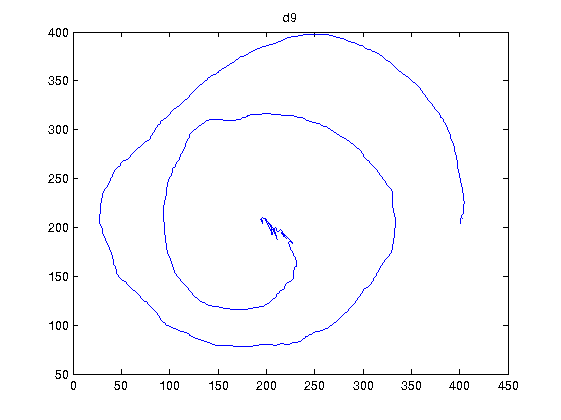
\includegraphics[scale = 1]{d9.png}
  \centering
  \caption{Example from one of the csv files}\hspace*{\fill}
  \label{fig:a}
\end{figure}


The key part here is that it affects the motor system, and as we all know it generates tremors, this is particularly obvious in the hands. Now, let's reflect on that. If someone with tremor in the hand tries to draw a straight line we will probably get something that looks more like a shaw edge, since the tremor will make the pen move in a more erratic fashion. Comparing this to what a straight line drawn by a healthy person would look like, if we say that the line is horizontal we would see a bigger variance in Y axis from the parkinson drawing. This will be one of the metrics I will be using.

Nonetheless I am working with spirals and circles which have the added feature at any given point the direction at which the pen has to move is different since the tangent for any given point of a circle is different so I will have to take into account the variance of at the very least X and Y, Z, although if you look at the Z in the files it is mostly 0 it does serve as a decent flag since people with parkinson are more likely to have variance in that value so I decided to include it and it does in fact give me better results than when taking it out. 

\bigskip

Since we already concluded that the tremors will generate more inconsistent drawings in the X, Y and Z axis it is important to notice that this will also affect the pressure that you are applying to the tablets and the angle at which you hold the pen so we will also take into account the variance for this values.

So far I have 5 features. Well, since the main thing Parkinson disease causes in drawings is inconsistency another feature I can measure is  the difference between the highest value and the lowest.

This brings us to 10 features, I will only add one more, since we have different types of tests I will also take this into account.

\subsection{Description of the approach}

\begin{enumerate} 
 
  \item Access the folders where the data is stored.
	\item For every file in the directory we split it by the test\_id
	\item Each part of the previous split gets split again in an arbitrary number of subsets.
	\item For every subset of the data we compute the variance and the difference for the mentioned features and store the test type.
	\item Getting the classes
\end{enumerate} 

\subsection*{First acces the folders:}

I used Glob to get a list of all the files ending in “.txt” of the folder with the mentioned path. For each file there is on the folder I read it using pandas and store it as a pandas DataFrame.
\bigskip
\bigskip
\subsection*{Splitting the files:}

This is a fairly simple task we iterate through the dataframe and as long as the test type is the same we add it to a list, as soon as the test changes we end the previous list save as a DatraFrame.
\bigskip
\bigskip
\subsection*{Splitting the test data:}

For this I used numpy to split each dataframe into X subsets. Here I also attempt to tackle a very important problem I face with this dataset. Since the amount of Parkinson cases is more than 4 times the amount of healthy cases I decided to do a skewed split of the dataset, meaning I will split the healthy cases in more subsets than the Parkinson cases. With the proper set up and with the proper feature selection we can avoid making massive difference in the amount of subsets. I decided to avoid making a split difference more than double between the two. In order to make this work properly it is better to make a large amount of subsets with numbers well into the hundreds, I have found that splitting the control data in 750 subsets while the parkinson data is split into 400 subsets yields very good results with very little training time. This will also give us a smaller variance in our subsets.

\begin{figure}[h!]
  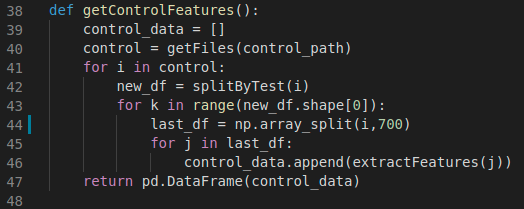
\includegraphics[scale = 1]{control.png}
  \centering
  \caption{function to get the all the feautres of the control data}\hspace*{\fill}
  \label{fig:a}
\end{figure}

\bigskip
\bigskip

\subsection*{Getting the features:}

For every subset of values we extract the variance and the difference of each column we are interested in as well as the test type. 
Getting the class

\subsection*{Getting the classes:}
In order to get the classes I create arrays of zeros and ones of the size corresponding to the amount of control and parkinson features stracted.

\bigskip
\bigskip
\bigskip
\bigskip
\section{Neural Network}

In order to solve this classification problem I am going to use a multilayer perceptron which is very commonly used supervised ML tasks. I have used both interchangeably a softmax function and a sigmoid function to perform the inference in the last layer. The prediction will be the maximum argument of this layer.
But before I will do a brief overview of how I set up the data to feed it to the NN.


How we feed the data to our NN will be one import thing that needs to be discussed. I have tried to main ways of doing this splits, so let's get into the first one

\subsection*{StratifiedKFold:}

This was suggested by  Roberto Santana so It was an obvious option to try out. Nonetheless it was a major disappointment. When using this way of splitting the data the NN needed more than eight times the time to train and ended up with 10\% worse accuracy.
\subsection*{Train\_test\_split:}

Using this way of splitting the data with a test size of 0.3 and the random state set to 30 the neural network was able to learn in a faster fashion and with better accuracy so I decided to use this way of splitting the data.

After getting the split done I one one hot encoded the classes so i can feed them to NN.

\subsection{NN structure}

I will expand on many things regarding the set up of the NN. Before I get into the specifics of each one I will point out that one of the recurrent factors in deciding the pieces I used was their capability of escaping local minima.

\subsection*{Layers:}

The first layer will have the same size as features we have, this is to say 11, and the last layer will have as many nodes as classes, 2. So we now have only to discuss how many hidden layers I am going to use in the perceptron, and as a matter of fact I will only use one, with 7 nodes in it. I have tried many different ways of setting up the hidden layers and out that using a single hidden layer of a size that lies in between the first layer and the last. Models that had this quality were faster in scaping local minima than models that had more hidden layers.
\bigskip
\subsection*{Loss function:}

I have tried many off the loss functions that are available in the tensorflow api and of the ones that are in keras, none of them were able to escape the local minimo that gave them accuracy higher than 0.70 and the ones that did immediately fell in the exact opposite local minima of getting all the control ones right and guessing none of the parkinson cases correctly.

I also tried out some of the loss functions that are available on the tensordflow.nn module, 2 of them stud out, both the sigmoid and the softmax cross entropy with logits, in case of the softmax the V2 version. These two were able to escape local minima pretty much from the starting point. Both work incredibly well with these set up and can be pretty much interchanged.

\subsection*{Optimizer:}

When it came to optimizers I once again decided to try many of the ones that are available directly in tensorflow. My main goal was to use the stochastic gradient descent (SGD), but having the tensorflow v2 behaviour dissabled made the module inaccessible and couldn't make it work. As for the others onces again the same problem. Since predicting all the cases to be Parkinson cases gives a great accuracy and its a local minima not far away from the absolute minima, many of them were unable to escape this minima no matter the epochs and no matter the learning rate. The only optimizer that was able to give good results not only escaping local minima but doing it very fast was the Adam optimizer.

\subsection*{Mini\_batch\_size:}

Even though this is not a major point in the MLP, I want to point out that finding an appropriate size for the mini batch did help the network reach an optimal point faster.


\bigskip
\subsection{Results}

Using a random train test split at 30\% test rate, one hidden layer of size 7, the sigmoid cross entropy with logits loss function, the adamp optimizer with a learning rate of 0.0005 and splitting the the control and parkinson data in 700 and 400 subsets this are the results that I have been able to achieve.

Escape local minima before 2000 epochs, after 14k epochs an accuracy of 0.84 with the same number of errors in both classes.
\begin{figure}[h!]
  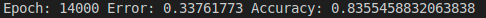
\includegraphics[scale = 1]{epoch14.png}
  \centering
  \caption{Results of the previous NN}\hspace*{\fill}
  \label{fig:a}
\end{figure}

Similar results can be obtained with two hidden layers sizes 9 and 4 a learning rate of 0.00005 and 150k epochs but since it takes 10 times more epoch to reach the same result I decided to discard this possibility. 

\begin{figure}[h!]
  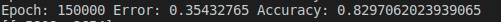
\includegraphics[scale = 1]{epoch150.png}
  \centering
  \caption{Results of the new NN}\hspace*{\fill}
  \label{fig:a}
\end{figure}

\bigskip
\bigskip
\bigskip
\bigskip
\bigskip
\bigskip
\bigskip
\bigskip

You can get even better results if your splits are even more disproportionate towards the control even up to 0.96 accuracy but this tampers with the data too much.

\bigskip

Lets take a look a t the confusion matrixes of the first two MLPs
\begin{table}[!h]
\centering
\begin{tabular}{lrrrr}
\toprule \hline
col\_0 &   0 &   1 & \\\hline
0     &  5545 &   2230 & \\\hline
1     &   2304 &  17491  \\\hline
\bottomrule \hline
\end{tabular}
\caption{Confusion Matrix for the MLP perceptron with only one hiden layer}
 \label{tab:CG}
\end{table}

\begin{table}[!h]
\centering
\begin{tabular}{lrrrr}
\toprule \hline
col\_0 &   0 &   1 & \\\hline
0     &  5808 &   2654 & \\\hline
1     &   2041 &  17067  \\\hline
\bottomrule \hline
\end{tabular}
\caption{Confusion Matrix for the MLP perceptron with two hiden layers}
 \label{tab:CG}
\end{table}
\bigskip
\bigskip
\bigskip
\bigskip
\bigskip
\bigskip


The biggest problem with the second NN is that it classifies por sick people as healthy on top of taking 10 times more time to train so I would recommend using the first one. The biggest problem with getting a better accuracy at this point is not the dataset as I have shown the NN is quite capable of performing well despite the imbalances present. At this point the main issue is the data, There is not enough of a big difference when comparing the numbers that both healthy people and sick people give us.
\bigskip


\bigskip
\section{Different Approach to feature selection and the NN}

I mentioned before in this document that I didn't think that splitting the data in different sizes was the correct approach, this is especially a problem when the test data is being split along with train data. So I tried a different approach to both preprocessing the data and setting up the neural network. It does take longer to trayn since the data set and validation are a bit trickier but the results are worth it.

\subsection*{Feature Selection}

To begin with the training data will have to continue with different splits 70 and 40 respectively but the test data will be split in the same manner for both classes, 40 splits per test type. So there is no bias in the testing part of the problem. This way we have balanced as much as we can our training data without compromising the testing data. Now the question remains if the NN can help us solve this problem.

\subsection*{NN with varying learning rate}

I have made small but crucial changes to how our MLP operates, in order to be able to solve this problem a regular NN has problems since the differences are small to begin with and the data is heavily Parkinson sided. In order to give the NN a bit more versatility I have implemented my own “momentum”. Since the number of epochs has to go up to accommodate the new complexity I can easily implement a varying learning rate. The neural network will start with what could be considered a “high” learning rate starting at 0.005 and every 250k epoch the learning rate decreases the value linearly. This gives the NN the ability to escape the part where it only predicts Parkinson cases and after it gets out fine tune to get a better accuracy. 

\begin{figure}[h!]
  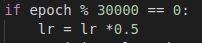
\includegraphics[scale = 1]{varlr.png}
  \centering
  \caption{Varying learning rate}\hspace*{\fill}
  \label{fig:a}
\end{figure}


The inverse way does also work similarly. Starting with a slow learning rate and increasing it. This gives similar results

With this new set up it is actually easily observable what the NN is learning, in the beginning it is stuck with the parkinson cases, but eventually it realizes that it is misclassifying many control cases and it will start to degrade itś accuracy before going once more back up this time correctly classifying more control cases.
\bigskip
\bigskip

\subsection*{Results}

This new approach gets similar results with an accuracy of 0.811 which is not far from the best results of the original approach but it doesn't disturb the quality of the testing data at all. Not only the accuracy is great but the confusion matrix shows that it also minimizes the error in diagnosing sick patients as healthy ones.
\bigskip
\bigskip

\begin{figure}[h!]
  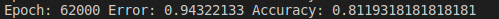
\includegraphics[scale = 1]{epoch292.png}
  \centering
  \caption{MLP defined in sklearn}\hspace*{\fill}
  \label{fig:a}
\end{figure}

\bigskip
\bigskip
\bigskip
\bigskip
\bigskip
\begin{table}[h!]
\centering
\begin{tabular}{lrrrr}
\toprule \hline
col\_0 &   0 &   1 & \\\hline
0     &  153 &   84 & \\\hline
1     &   247 &  1276  \\\hline
\bottomrule \hline
\end{tabular}
\caption{Confusion Matrix for the NN with varying learning rate}
 \label{tab:CG}
\end{table}

\bigskip
\bigskip
\bigskip
\bigskip
\bigskip
\bigskip
\bigskip
\bigskip
\bigskip
\bigskip
\section{Restricted Boltzzman machine}

This was the last approach I took to solve the problem. I decided to use sklearns BernoulliRBM and create a pipeline with it and the MLP.

\bigskip
\subsection{Feature selection}

I will start talking about feature selection. The first approach I took was to feed the RBM the entire dataset with the labels. This didn't work at all for two main reasons, the first one is the fact that training a RMB with hundreds of thousands of cases, proved to be too computationally costly mainly because it runs on the processor, this got worse when I tried to learn 100+ features with each epoch taking up to 8 seconds. Further more after training the RBM from the original data with a number 100 components and 10k epochs the pipeline wasn't able to skip the local minima of predicting every case to be a Parkinson one. I tried to make a few adjustments to the whole process but after 5 tries that took more than 3h I decided this was not a feasible way of proceeding.

The next approach was to feed the RMB some of the selected features I used in  previous solutions. The difference being that both the parkinson and the control data would be split in 40 pieces, both the same amount to keep the integrity of the testing data. The features that were selected to feed the RMb was the total difference ignoring the variance and the test id since this gave the best results by far. 

As a final note I will point out that I tried these changes in the original NN and the results were quite worse compared to the original feature selection, the NN lost around .2 accuracy.
\bigskip

\subsection{BernoulliRBM}

I took this restricted Boltzmann machine from sklearn and set it up  in the following fashion:


\begin{itemize}
\item Learning rate = 0.0002
\item N\_iter = 300
\item N\_componets = 200 

\end{itemize}

Increasing the epochs or the number of components made little difference so I stuck with a way that at least made the training process fast enough.

\begin{figure}[h!]
  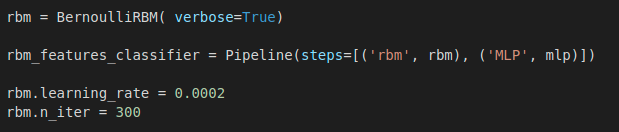
\includegraphics[scale = 1]{pipe.png}
  \centering
  \caption{Definition of the RBM and the pipeline}\hspace*{\fill}
  \label{fig:a}
\end{figure}

\bigskip
\bigskip
\bigskip
\bigskip
\bigskip
\subsection{MLPClassifier}

As I mentioned I used the sklearn MLP in order to make the process easier using a pipeline. I tried both the adam and the sgd solvers and ended up deciding to go with the adam optimizer since it gave slightly better results. The MLP trains for 5k epochs As for the activation function, the one that worked the best was the relu function. I decided to use the same learning rate of 0.0005 since it consistently performed better than the rest. I also added a  momentum of 0.7, it gave the best results. To finish up the details I will mention that after several tries setting up 2 hidden layers of sizes 70 and 10 was the best layer combination I found.

\begin{figure}[h!]
  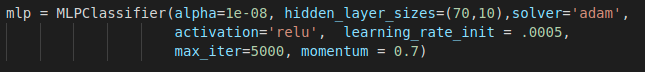
\includegraphics[scale = 0.7]{mlpsk.png}
  \centering
  \caption{MLP defined in sklearn}\hspace*{\fill}
  \label{fig:a}
\end{figure}



\bigskip

\subsection{Results}

The results obtained by this approach are comparable with the other two but, taking into account that  it does not put into a compromise the testing data like the first approach does I think these are inherently better results compared to those.

This pipeline managed and accuracy of 0.82.


\begin{figure}[h!]
  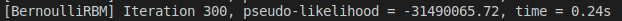
\includegraphics[scale = 0.7]{epoch300.png}
  \centering
  \caption{Function for changing the learning rate}\hspace*{\fill}
  \label{fig:a}
\end{figure}

Lets take a look at the confusion matrix

\begin{table}[!h]
\centering
\begin{tabular}{lrrrr}
\toprule \hline
col\_0 &   0 &   1 & \\\hline
0     &  10 &   3 & \\\hline
1     &   425 &  1986  \\\hline
\bottomrule \hline
\end{tabular}
\caption{Confusion Matrix for the pipeline with of the RMB and the MLP}
 \label{tab:CG}
\end{table}
\bigskip
\bigskip

\section{Implementation}
This project was implemented in python3 in Windows10 but it is perfectly compatible with linux since the packages are the same for both systems. All the implementation can be found in the folder with the name code, there you can also find Jupyter notebooks explaining the code. This hole project is also available in github and is accessible by this link:
\smallskip

https://github.com/Canis-Ignem/Parkinson-Detection-ShallowNN


\bigskip
\bigskip
\bigskip
\bigskip
\bigskip
\bigskip
\bigskip
\bigskip
\bigskip
\bigskip

\section{Conclusions}

The first thing I want to mention here is that tampering with the testing data should not be done if you want your ML solution to achieve regularization. This is the main reason I discard the first solution presented in this paper. Now coming to talk about the other two solutions, Both of them keep the integrity of the data and give very similar and good results. Those twoo solutions stand as proof that if defined properly and with the appropriate feature engineering even an unbalanced dataset can be primed for machine learning.
\section{Documentation} 

I did not have to read any literature on the subject in order to reach this solution. I have mentioned the Deep Learning book becouse I did indeed read it, but it was more than a year ago. So all this solution is extrictly my own.

\begin{enumerate} 

\item DeepLearning - Goodfellow

\item Tensorflow r1.15 - https://www.tensorflow.org/versions/r1.15/api\_docs/python/tf 
 
\item Sklearn: https://scikit-learn.org/stable/index.html



\end{enumerate} 
\end{document}
